% This is "sig-alternate.tex" V2.1 April 2013
% This file should be compiled with V2.5 of "sig-alternate.cls" May 2012
%
% This example file demonstrates the use of the 'sig-alternate.cls'
% V2.5 LaTeX2e document class file. It is for those submitting
% articles to ACM Conference Proceedings WHO DO NOT WISH TO
% STRICTLY ADHERE TO THE SIGS (PUBS-BOARD-ENDORSED) STYLE.
% The 'sig-alternate.cls' file will produce a similar-looking,
% albeit, 'tighter' paper resulting in, invariably, fewer pages.
%
% ----------------------------------------------------------------------------------------------------------------
% This .tex file (and associated .cls V2.5) produces:
%       1) The Permission Statement
%       2) The Conference (location) Info information
%       3) The Copyright Line with ACM data
%       4) NO page numbers
%
% as against the acm_proc_article-sp.cls file which
% DOES NOT produce 1) thru' 3) above.
%
% Using 'sig-alternate.cls' you have control, however, from within
% the source .tex file, over both the CopyrightYear
% (defaulted to 200X) and the ACM Copyright Data
% (defaulted to X-XXXXX-XX-X/XX/XX).
% e.g.
% \CopyrightYear{2007} will cause 2007 to appear in the copyright line.
% \crdata{0-12345-67-8/90/12} will cause 0-12345-67-8/90/12 to appear in the copyright line.
%
% ---------------------------------------------------------------------------------------------------------------
% This .tex source is an example which *does* use
% the .bib file (from which the .bbl file % is produced).
% REMEMBER HOWEVER: After having produced the .bbl file,
% and prior to final submission, you *NEED* to 'insert'
% your .bbl file into your source .tex file so as to provide
% ONE 'self-contained' source file.
%
% ================= IF YOU HAVE QUESTIONS =======================
% Questions regarding the SIGS styles, SIGS policies and
% procedures, Conferences etc. should be sent to
% Adrienne Griscti (griscti@acm.org)
%
% Technical questions _only_ to
% Gerald Murray (murray@hq.acm.org)
% ===============================================================
%
% For tracking purposes - this is V2.0 - May 2012

\documentclass{sig-alternate}
\usepackage[numbers]{natbib}
\usepackage{listings}
% Handle Images
\makeatletter
\def\maxwidth{\ifdim\Gin@nat@width>\linewidth\linewidth\else\Gin@nat@width\fi}
\def\maxheight{\ifdim\Gin@nat@height>\textheight\textheight\else\Gin@nat@height\fi}
\makeatother
% Scale images if necessary, so that they will not overflow the page
% margins by default, and it is still possible to overwrite the defaults
% using explicit options in \includegraphics[width, height, ...]{}
\setkeys{Gin}{width=\maxwidth,height=\maxheight,keepaspectratio}

% Hyper-references
\usepackage{hyperref}
\hypersetup{unicode=true,
            pdftitle={Studying Software Design as Students Learn to Program},
            pdfauthor={{[}Blinded for Review{]}},
            pdfborder={0 0 0},
            breaklinks=true}
\urlstyle{same}  % don't use monospace font for urls

% Syntax Highlighting
\usepackage{color}
\usepackage{fancyvrb}
\newcommand{\VerbBar}{|}
\newcommand{\VERB}{\Verb[commandchars=\\\{\}]}
\DefineVerbatimEnvironment{Highlighting}{Verbatim}{commandchars=\\\{\}}
% Add ',fontsize=\small' for more characters per line
\newenvironment{Shaded}{}{}
\newcommand{\KeywordTok}[1]{\textcolor[rgb]{0.00,0.44,0.13}{\textbf{{#1}}}}
\newcommand{\DataTypeTok}[1]{\textcolor[rgb]{0.56,0.13,0.00}{{#1}}}
\newcommand{\DecValTok}[1]{\textcolor[rgb]{0.25,0.63,0.44}{{#1}}}
\newcommand{\BaseNTok}[1]{\textcolor[rgb]{0.25,0.63,0.44}{{#1}}}
\newcommand{\FloatTok}[1]{\textcolor[rgb]{0.25,0.63,0.44}{{#1}}}
\newcommand{\ConstantTok}[1]{\textcolor[rgb]{0.53,0.00,0.00}{{#1}}}
\newcommand{\CharTok}[1]{\textcolor[rgb]{0.25,0.44,0.63}{{#1}}}
\newcommand{\SpecialCharTok}[1]{\textcolor[rgb]{0.25,0.44,0.63}{{#1}}}
\newcommand{\StringTok}[1]{\textcolor[rgb]{0.25,0.44,0.63}{{#1}}}
\newcommand{\VerbatimStringTok}[1]{\textcolor[rgb]{0.25,0.44,0.63}{{#1}}}
\newcommand{\SpecialStringTok}[1]{\textcolor[rgb]{0.73,0.40,0.53}{{#1}}}
\newcommand{\ImportTok}[1]{{#1}}
\newcommand{\CommentTok}[1]{\textcolor[rgb]{0.38,0.63,0.69}{\textit{{#1}}}}
\newcommand{\DocumentationTok}[1]{\textcolor[rgb]{0.73,0.13,0.13}{\textit{{#1}}}}
\newcommand{\AnnotationTok}[1]{\textcolor[rgb]{0.38,0.63,0.69}{\textbf{\textit{{#1}}}}}
\newcommand{\CommentVarTok}[1]{\textcolor[rgb]{0.38,0.63,0.69}{\textbf{\textit{{#1}}}}}
\newcommand{\OtherTok}[1]{\textcolor[rgb]{0.00,0.44,0.13}{{#1}}}
\newcommand{\FunctionTok}[1]{\textcolor[rgb]{0.02,0.16,0.49}{{#1}}}
\newcommand{\VariableTok}[1]{\textcolor[rgb]{0.10,0.09,0.49}{{#1}}}
\newcommand{\ControlFlowTok}[1]{\textcolor[rgb]{0.00,0.44,0.13}{\textbf{{#1}}}}
\newcommand{\OperatorTok}[1]{\textcolor[rgb]{0.40,0.40,0.40}{{#1}}}
\newcommand{\BuiltInTok}[1]{{#1}}
\newcommand{\ExtensionTok}[1]{{#1}}
\newcommand{\PreprocessorTok}[1]{\textcolor[rgb]{0.74,0.48,0.00}{{#1}}}
\newcommand{\AttributeTok}[1]{\textcolor[rgb]{0.49,0.56,0.16}{{#1}}}
\newcommand{\RegionMarkerTok}[1]{{#1}}
\newcommand{\InformationTok}[1]{\textcolor[rgb]{0.38,0.63,0.69}{\textbf{\textit{{#1}}}}}
\newcommand{\WarningTok}[1]{\textcolor[rgb]{0.38,0.63,0.69}{\textbf{\textit{{#1}}}}}
\newcommand{\AlertTok}[1]{\textcolor[rgb]{1.00,0.00,0.00}{\textbf{{#1}}}}
\newcommand{\ErrorTok}[1]{\textcolor[rgb]{1.00,0.00,0.00}{\textbf{{#1}}}}
\newcommand{\NormalTok}[1]{{#1}}
\usepackage{longtable,booktabs}
\usepackage{graphicx,grffile}

% pandoc's tightlist
\providecommand{\tightlist}{%
  \setlength{\itemsep}{0pt}\setlength{\parskip}{0pt}}

\begin{document}

% Copyright
\setcopyright{acmcopyright}
%\setcopyright{acmlicensed}
%\setcopyright{rightsretained}
%\setcopyright{usgov}
%\setcopyright{usgovmixed}
%\setcopyright{cagov}
%\setcopyright{cagovmixed}


% DOI
\doi{10.475/123_4}

% ISBN
\isbn{123-4567-24-567/08/06}

%Conference
\conferenceinfo{PLDI '13}{June 16--19, 2013, Seattle, WA, USA}

\acmPrice{\$15.00}

%
% --- Author Metadata here ---
\conferenceinfo{WOODSTOCK}{'97 El Paso, Texas USA}
%\CopyrightYear{2007} % Allows default copyright year (20XX) to be over-ridden - IF NEED BE.
%\crdata{0-12345-67-8/90/01}  % Allows default copyright data (0-89791-88-6/97/05) to be over-ridden - IF NEED BE.
% --- End of Author Metadata ---

\title{Reconstructing design thinking and learning through code snapshots and clinical interviews}

%
% You need the command \numberofauthors to handle the 'placement
% and alignment' of the authors beneath the title.
%
% For aesthetic reasons, we recommend 'three authors at a time'
% i.e. three 'name/affiliation blocks' be placed beneath the title.
%
% NOTE: You are NOT restricted in how many 'rows' of
% "name/affiliations" may appear. We just ask that you restrict
% the number of 'columns' to three.
%
% Because of the available 'opening page real-estate'
% we ask you to refrain from putting more than six authors
% (two rows with three columns) beneath the article title.
% More than six makes the first-page appear very cluttered indeed.
%
% Use the \alignauthor commands to handle the names
% and affiliations for an 'aesthetic maximum' of six authors.
% Add names, affiliations, addresses for
% the seventh etc. author(s) as the argument for the
% \additionalauthors command.
% These 'additional authors' will be output/set for you
% without further effort on your part as the last section in
% the body of your article BEFORE References or any Appendices.

\numberofauthors{8} %  in this sample file, there are a *total*
% of EIGHT authors. SIX appear on the 'first-page' (for formatting
% reasons) and the remaining two appear in the \additionalauthors section.
%
\author{
% You can go ahead and credit any number of authors here,
% e.g. one 'row of three' or two rows (consisting of one row of three
% and a second row of one, two or three).
%
% The command \alignauthor (no curly braces needed) should
% precede each author name, affiliation/snail-mail address and
% e-mail address. Additionally, tag each line of
% affiliation/address with \affaddr, and tag the
% e-mail address with \email.
%
% 1st. author
\alignauthor
% Ben Trovato\titlenote{Dr.~Trovato insisted his name be first.}\\
%        \affaddr{Institute for Clarity in Documentation}\\
%        \affaddr{1932 Wallamaloo Lane}\\
%        \affaddr{Wallamaloo, New Zealand}\\
%        \email{trovato@corporation.com}
Authors Blinded For Review
}
\maketitle
\begin{abstract}

\end{abstract}


%
% The code below should be generated by the tool at
% http://dl.acm.org/ccs.cfm
% Please copy and paste the code instead of the example below.
%
\begin{CCSXML}
<ccs2012>
 <concept>
  <concept_id>10010520.10010553.10010562</concept_id>
  <concept_desc>Computer systems organization~Embedded systems</concept_desc>
  <concept_significance>500</concept_significance>
 </concept>
 <concept>
  <concept_id>10010520.10010575.10010755</concept_id>
  <concept_desc>Computer systems organization~Redundancy</concept_desc>
  <concept_significance>300</concept_significance>
 </concept>
 <concept>
  <concept_id>10010520.10010553.10010554</concept_id>
  <concept_desc>Computer systems organization~Robotics</concept_desc>
  <concept_significance>100</concept_significance>
 </concept>
 <concept>
  <concept_id>10003033.10003083.10003095</concept_id>
  <concept_desc>Networks~Network reliability</concept_desc>
  <concept_significance>100</concept_significance>
 </concept>
</ccs2012>
\end{CCSXML}

\ccsdesc[500]{Computer systems organization~Embedded systems}
\ccsdesc[300]{Computer systems organization~Redundancy}
\ccsdesc{Computer systems organization~Robotics}
\ccsdesc[100]{Networks~Network reliability}


%
% End generated code
%

%
%  Use this command to print the description
%
\printccsdesc

% We no longer use \terms command
%\terms{Theory}

\keywords{ACM proceedings; \LaTeX; text tagging}

\section{Introduction}

\section{Introduction}\label{introduction}

A growing trend in computer science education research is the collection and analysis of code snapshot data--records of the state of and changes to students' code as they develop it \cite{jadud_methods_2006,rodrigo_analyzing_2009,spacco_marmoset_2006}. Though specific implementations differ, the general strategy in such projects is that a student event (typically compiling code or saving a file) triggers a procedure that creates a record containing the entire content of all of a student's relevant files, as well as associated metadata (time of save/compilation, for example, and any compiler errors that may have been generated). Mining data from such snapshotting systems has led to large-scale documentation of common student errors \cite{spacco_marmoset_2006}, the development of compile-time detectors to catch common student errors \cite{spacco_software_2005}, and the proposal of formative assessment models to predict student success \cite{jadud_methods_2006,tabanao_predicting_2011}. Building on existing momentum, some researchers are actively pushing for a continued scale-up of how we collect code snapshot data. One current proposal even calls for creating an international database by collecting snapshot data from thousands of introductory programming students worldwide \cite{kolling_building_2012}.

What's common to these threads of research is how they mine the data. In
most applications of code snapshot\footnote{What I call ``code
  snapshot'' research may be more formally called ``online protocol''
  research \cite{jadud_methods_2006,rodrigo_analyzing_2009}. ``Online'' here isn't mean to mean
  the sense of globally-connected computers, but rather that student
  materials are collected in a minimally-intrusive way \emph{while
  students work}.} research, the aim is to average across events and
sessions to arrive at a characteristic measure of a student's behavior.
Jadud \cite{jadud_methods_2006}, for example, develops the idea of a student's ``Error
Quotient,'' a measure of how effectively a student addresses
compile-time errors in their code.\footnote{A useful way of thinking
  about Jadud's \cite{jadud_methods_2006} error quotient is that the computation believes
  in second chances. It doesn't penalize students for making errors; it
  penalizes students if they don't fix a given error before compiling
  the same piece of code \emph{again.}} Rodrigo and colleagues extend
the idea of error quotient and introduce similar
measures such as students' ``compilation profiles'' \cite{rodrigo_analyzing_2009}, ``frustration profiles'' \cite{rodrigo_affective_2009}, and ``error
profiles'' \cite{tabanao_predicting_2011}. Because these measures can be
collected in real-time as students code, they offer the potential to
identify at-risk students and respond with early
interventions.

But, for all the data these methods collect their focus is primarily
what Jadud \cite{jadud_methods_2006} calls students' ``syntactic'' struggles: the challenge
of articulating well-formed statements a compiler can properly parse.
This focus on syntax-level struggles leads to both a methodological and
theoretical trade-off: we can see in detail how students struggle with
wording, but we see less of how they struggle with the meaning and
intent of their code. Syntactical analyses necessarily ignore the
specific \emph{content} of students' code because they abstract
meta-information about the event: error type, error location, frequency
of error.

As an analogy, suppose that instead of studying computer science
students we were studying screenwriting students. Further suppose we
have a system to track data whenever students save their screenplays and
scripts. For each save, we get a copy of the entire script at that time.
We can also run an automated analysis to check whether they've properly
formatted slug lines\footnote{In a screenplay, a slug line gives
  information about where and when a scene takes place. For example:
  \texttt{``INT. FORTRESS OF SOLITUDE -- DAY.''}}, put character names in
all-capital letters, properly numbered scenes, etc. We might even know
where students are when they write (coffee shop, library, home, etc.).
If we mine that data, we could learn something about students'
\emph{screenwriting behavior}, but only at the level of how they
struggle with screenwriting syntax. Using only error-based data it's
much harder to answer questions such as:

\begin{itemize}
  \tightlist
\item
  How does this student construct a scene or handle dialog in their
  script?
\item
  Does the student seem to have a grasp of pacing, story beats, and
  efficient exposition?
\item
  How does their writing manage and develop character arcs?
\end{itemize}

We also still can't answer fundamental questions about the context of
students' writing processes:

\begin{itemize}
  \tightlist
\item
  Do they use particular techniques to ``break story'' and decompose a
  narrative into its key beats (index cards? Whiteboard?)
\item
  Do they participate in a writing group?
\item
  How do they respond to people giving them notes on revising a script?
\end{itemize}

To sum up, because snapshot systems are designed to collect the totality
of a codebase at frequent intervals, they offer a rich record of data
that captures the results---both major and minor---of students' design
decisions. But, computing education research that \emph{uses}
code-snapshotting has focused much more on detecting, classifying, and
predicting student errors than it has on showing how students progress
in programming and design expertise. Nevertheless, snapshot-based
research shows tremendous promise. Given that :

\begin{enumerate}
\def\labelenumi{\arabic{enumi}.}
\tightlist
\item
  Snapshotting students' code represents a cutting-edge way to resolve
  the way code---as a design artifact---evolves over time, \emph{but}
\item
  Code snapshots, as they're currently used, explore neither the
  totality of a student's design nor the rich context of that design's
  production, \emph{and}
\item
  There is a lack of parity between studies of how professionals design
  software and studies of how students do so,
\end{enumerate}

It seems sensible to ask: \emph{can code snapshots be used---possibly in
synthesis with ethnographically-oriented methods---to start studying how
students' design thinking plays a role in their introductory programming
work?} We believe the answer is yes.

In what follows, we present work that proceeds from an empirical
challenge: how can we develop accounts of students' programming activity
that explain the form and evolution of their code on a design project?
We offer an account of one student---Rebecca---and her experiences and
code from a second-semester course on programming concepts for
engineers. Using data from both code snapshots and clinical interviews,
we explicate both the challenges of studying students' software design
processes and the potential for such study to inform accounts of
teaching and learning.

\section{Context and Methods}\label{context-and-methods}

\subsection{Context of the study}\label{context-of-the-study}

The data presented in this case are taken from an ongoing IRB-approved
study of undergraduate electrical engineering majors undertaken at
\emph{Flagship State}, a large, public research institution on the east
coast. For two semesters, I have followed a total of 10 students taking
``Intermediate Programming Concepts for Engineers.'' It is the second of
a required two-semester course sequence in programming.\footnote{Hereafter,
  I use ``Intermediate Programming'' to refer to the second course and
  ``Basic Programming'' to refer to the first.} Students can (and some
do) place out of Basic Programming via AP Computer Science credit, but
all Electrical and Computer Engineering students must take Intermediate
Programming.

Intermediate Programming has two 75-minute lectures per week and a
weekly discussion section led by an undergraduate Teaching Assistant
(TA). Typical enrollment is between 60 and 80 students per semester.
Like Basic Programming, Intermediate Programming is taught using the C
programming language, and it incorporates multi-week projects in C as
part of its assessment structure. Students must work individually on
four projects over the course of the semester, which together comprise
45\% of their final course grade.

Grading projects involves running students' compiled code against
automated tests that determine whether a student program's output
matches the instructor's canonical output. If a student's program
completely matches the canonical output, the student receives at least a
90\% grade on a project. The remaining 10\% are discretionarily
allocated ``style'' points, awarded for things like proper formatting,
code commenting, and functional decomposition (Field Notes).

This study centers on ``Flights Database,'' the second of four projects
assigned to Intermediate Programming students during the spring 2012
semester. Students were asked to build a text menu-based program that
would let users query information about airports and plan non-stop and
one-stop flights between airports. For this project, the instructor gave
students three separate text files as source material. The
\textbf{airports} file contained names of airports and their
three-letter abbreviation codes; the \textbf{routes} file contained
3-tuples of two airport codes and the route number of a flight flying
between them; the \textbf{flights} file contained a list of specific
flight information (including arrival and departure times) by route
number. Crucially, in order to be able to respond to user queries
students would need to build a program that could coordinate information
across all three files to return an answer.

My analysis details the work of Rebecca, a female first-year electrical
engineering major. I focus specifically on Rebecca's code for finding
``one-stop'' flights, which the instructor defined as ``all pairs of
flights that route the user between the departure and arrival airports
with exactly 1 stop (i.e., a one-connection flight)'' (Flights Database
handout, 2012). The one-stop problem is particularly challenging. To
solve it successfully students' code must accept a user's choice of
airports and day, then stitch together routes that involve two separate
flights in a way that passes stringent constraints for acceptable
layover times.

\subsection{Methods}\label{methods}

This study proceeds from an empirical challenge: how can we develop
accounts of students' programming activity that explain the form and
evolution of their code on a design project? The focused form of that
challenge for this study is ``how can we understand the unconventional
design choices embedded in Rebecca's one-stop flight code?'' To answer
that question, my study draws from three data streams: ethnographic
observation, clinical interviewing, and code snapshot analysis.

For two semesters, I ethnographically embedded myself in the same
instructor's section of Intermediate Programming. My aim throughout was
to see what students see in terms of course material, assignment
directives, and instruction. In fall 2011 I observed approximately 50\%
of the course lectures. I also independently completed all class
homeworks and three out of the four course projects to more fully
understand the course's assessments. In spring 2012 I continued
attending lectures, though less frequently, and began attending select
TA-led discussion sections. During both lectures and discussion sections
I took field notes while recording ambient audio using a LiveScribe
Pulse pen.

Rebecca was one of four students (three female, one male) willing and
able to participate in a series of 1-hour outside-of-class clinical
interviews during the spring 2012 semester.\footnote{In total, roughly
  30 students responded to my initial in-class solicitation to be
  contacted by email about my study. Of the students I emailed,
  approximately 8 students responded to my emails to schedule interview
  times. Of those 8, only four students were able to successfully find
  interview time slots that fit our respective schedules.} I interviewed
Rebecca five times, and in typical interviews I split time between
asking about her experiences in the course and giving her time in the
interview to work on her project code. During each interview, I
simultaneously used:

\begin{enumerate}
\def\labelenumi{\arabic{enumi}.}
\tightlist
\item
  A Kodak Zi8 camera for video-recording our interactions
\item
  A LiveScribe Pulse pen to capture Rebecca's on-paper penstrokes
\item
  A MacBook Pro (early 2011) with screen-recording software to capture
  everything on-screen while Rebecca programmed
\end{enumerate}

The final component of data gathering is modeled after Jadud's (2006)
system for capturing students' code. My colleagues and I developed
software, built around the open-source version control system called
Git, that effectively creates an entire copy of a student's code---what
we call ``snapshots''---every time students invoke the compiler on their
code. Our software then sends those snapshots to a secure,
researcher-accessible server in real-time as they're created.
Consequently, I could plan each interview with Rebecca around
up-to-the-minute knowledge of her work---in some cases work she had
completed just hours before the interview---and tailor my interview
questions to emerging patterns in her code. In total, Rebecca's work
resulted in 958 compilation snapshots over the course of the semester.

\section{Analyzing only the code Rebecca turned in}\label{analyzing-only-the-code-rebecca-turned-in-what-an-instructor-might-see}

In this phase of analysis, I restrict data to only the final version of \texttt{one\_stop\_flight.c} Rebecca submitted as part of her project. This restriction is important because of the data that gets left out. We're forced to see Rebecca's design work the way her instructor did when he graded it: as a final product. The submitted code contains little---if any---evidence of design iteration. And, we have almost no access to streams of activity (inscriptional, gestural, verbal, and otherwise material) that would help us understand Rebecca's early stage design \citep{petre_software_2014}. Indeed, other than the code itself, the only artifacts that actually carry Rebecca's voice in this phase of analysis are the comments she places in her code. Put another way: restricting our scope to just code---and only the final submitted code at that---denies the analyst access to the channels of ``talk, embodied action, and inscription'' involved in design work \citep[ p.~179]{hall_disrupting_2002}.

\begin{figure}[htbp]
\centering
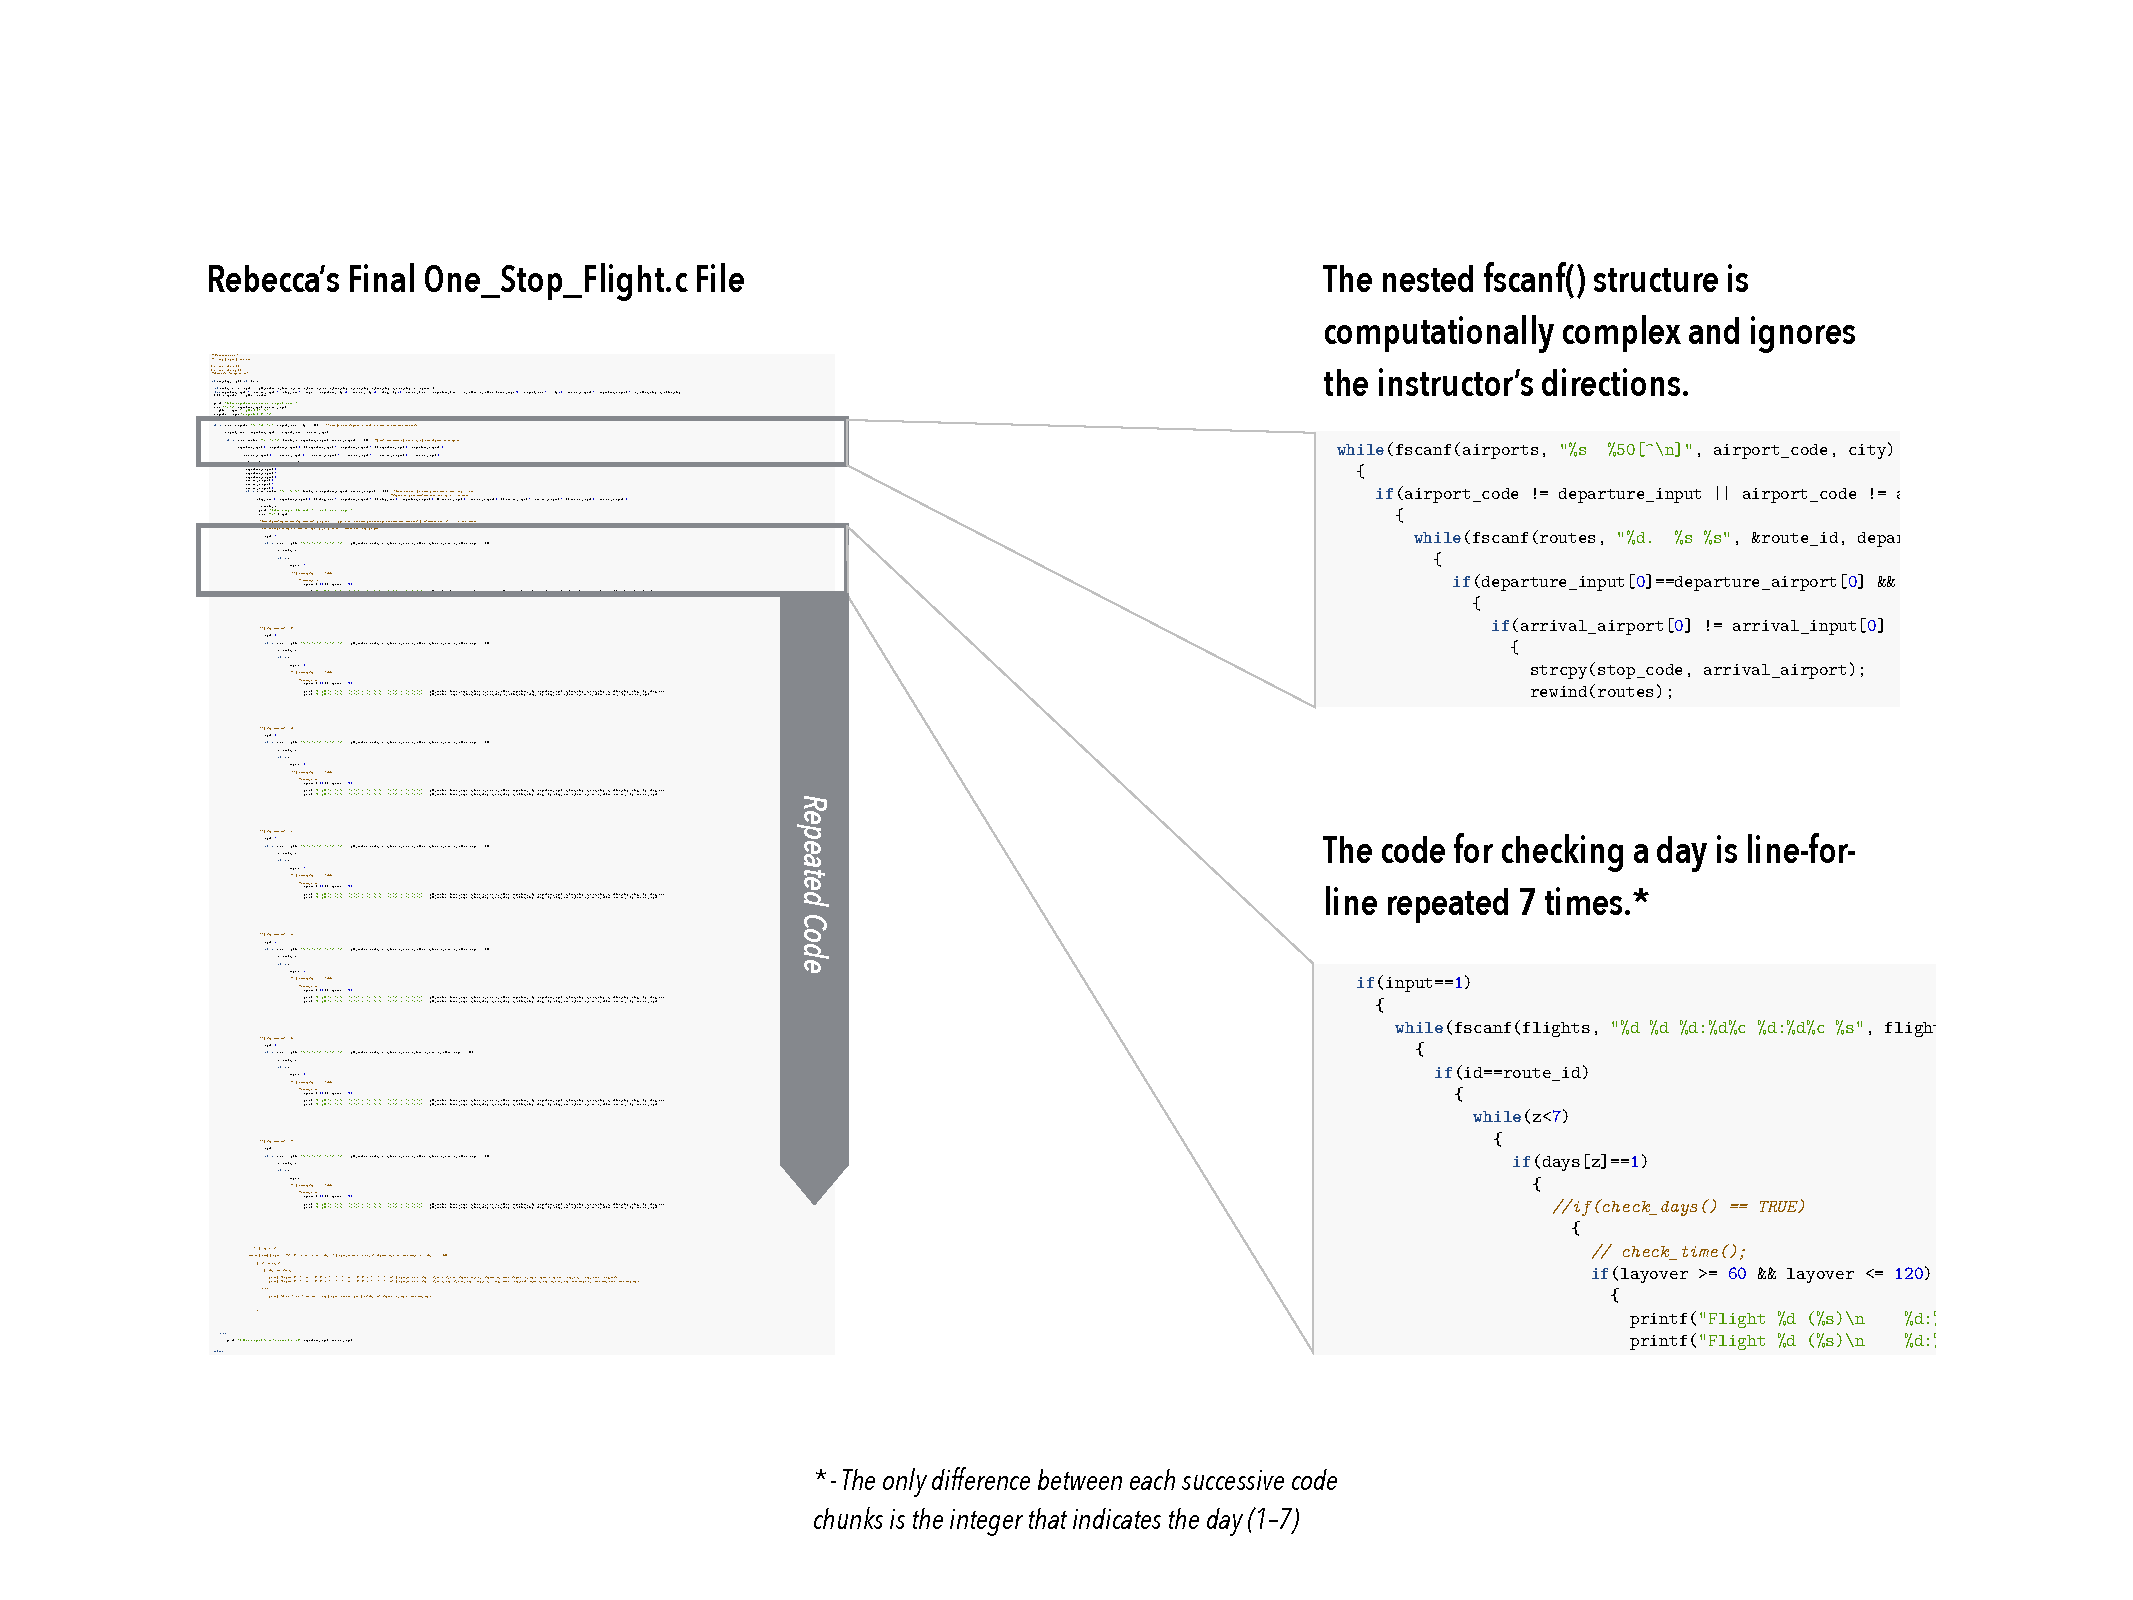
\includegraphics{RebeccasCode/OneStopFlightSupergraphic.pdf}
\caption{The entirety of Rebecca's \texttt{one\_stop\_flight.c} source code at the time her project was submitted for grading. Our final-code-only analysis focuses on two design features of this code: its multiply-nested \texttt{fscanf()} structure for handling flight data; and the seven-fold line-for-line repetition of a single block of code for checking days of the week.}
\end{figure}

\subsection{Rebecca's file-scanning solution is hard to read and has high time-complexity}\label{rebeccas-file-scanning-solution-is-hard-to-read-and-has-high-time-complexity}

After declaring variables and opening the three provided text files (flights, routes, and airports)\footnote{See Appendix A for examples of each of the three file types.}, Rebecca's one-stop flight code enters a series of conditionally-nested \texttt{fscanf()} commands. Any suitable solution for this project would need extract text patterns from source files, which \texttt{fscanf()} does. So, \emph{that} Rebecca uses \texttt{fscanf()} in her code is not itself surprising. Rather, what's interesting is \emph{how} she uses \texttt{fscanf()} in her design.

Rebecca's file-scanning logic never persistently stores the contents of the files it reads in. Rather, her program reads through files one line at a time, and it essentially can't process or act on airport/flight information not in the line currently being scanned. Instead, it's been designed to copy single patterns temporarily, then rewind the file back to the top and start reading in one-line-at-a-time again.

What's consequential about Rebecca's design choice? Computationally, her code has to repeatedly open multiple files (or sometimes repeatedly open the same file multiple times) and scan lines one line at a time in order to coordinate information. So, the task of finding a one-stop flight between two cities becomes a series of repeated, one-line-at-a-time scans of external files:

\begin{figure}[htbp]
\centering
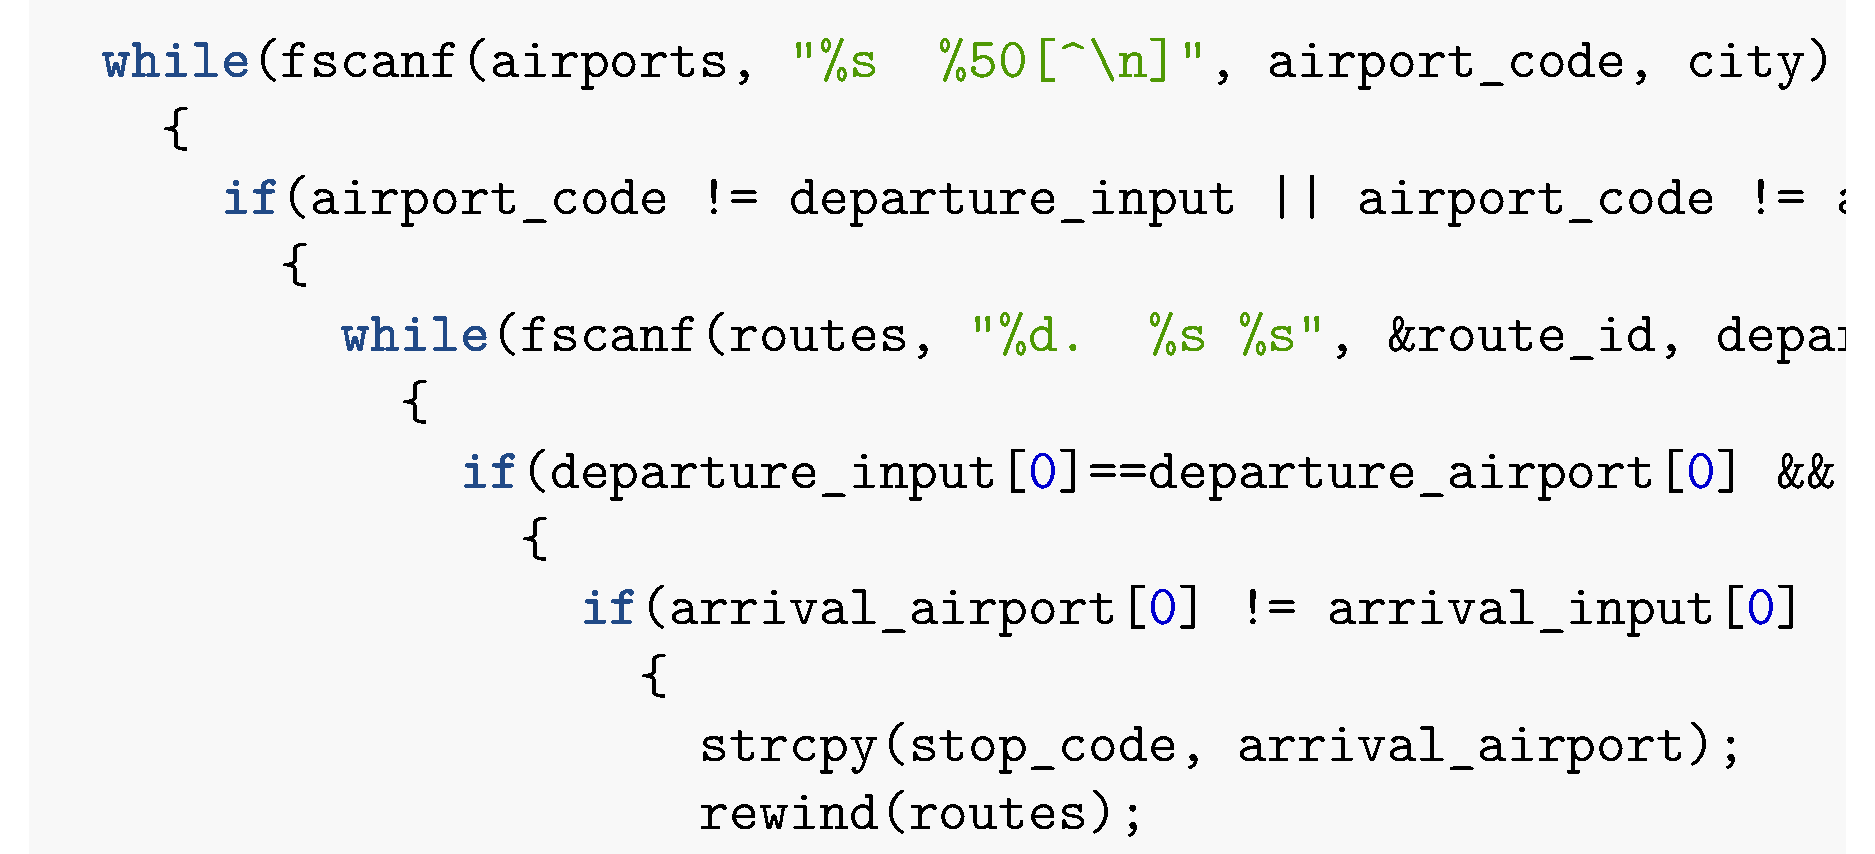
\includegraphics{media/fscanf.pdf}
\caption{A portion of Rebecca's nested \texttt{fscanf()} statements}
\end{figure}

\begin{enumerate}
\def\labelenumi{\arabic{enumi}.}
\tightlist
\item
  Scan the \textbf{airports} file one line at a time (line 20)
\item
  While scanning a given line containing an airport code/city pair, scan the file of pairwise airport \textbf{routes} one line at a time (line 24).
\item
  To find possible connection cities, scan the \textbf{routes} file one line at a time again (line 38)
\item
  If a route matches, scan the \textbf{flights} file one line at a time to verify whether the time/day constraints are acceptable (one of the following lines depending on the chosen day: 52, 79, 106, 134, 162, 190, 218).
\end{enumerate}

Rebecca's code is both visually and computationally complex. The multiply-nested blocks can make it difficult for a human reader (or grader) to follow the code flow, which may have made it challenging for Rebecca to debug her own work. Moreover, nested for- and while-loops increase dimensions of complexity in Rebecca's program---what computer scientists would call the ``Big-O'' characterization of her program \citep{cormen_introduction_1990}. For every nesting of a scan loop (there are 4 in her submitted code) Rebecca increases by 1 the degree of a polynomial that represents the execution time of her program. So, from a performance perspective, Rebecca's design suffers a trade-off in that with each invocation of a scanning loop, we see a geometric increase in the time complexity of her program. But, Rebecca's code also has a particular kind of elegance.

\subsection{Rebecca's file-scanning solution has elegant constant space complexity}\label{rebeccas-file-scanning-solution-has-elegant-constant-space-complexity}

While Rebecca's design isn't optimized for speed, it uses drastically less memory than do other solutions (including the instructor's official solution). What Rebecca could have done (and what I'll discuss in a later section) is read the entire contents of all data files into RAM. I'll call that approach an \emph{in-memory} solution, because all of the flight information is loaded into memory. Instead, her solution stores only a handful of lines (4 at most) in memory at a time, leaving the rest \emph{on-disk}. An analogy helps clarify the difference.

If we think of the input files like a giant grocery list, an in-memory solution would be like having to put each list item into your cart before you go to check out. The longer the list gets, the bigger cart you'd need to collect every item on the list before checking out. Crucially, everything has to go into the cart before it can be purchased. If the grocery list very long, you may need multiple carts. If the list gets absurdly long you may even exhaust all carts in the store and still find yourself with an unfinished list.

Rebecca's \emph{on-disk} solution would be like restricting yourself to a single, small grocery basket, but taking as many trips as you need to get all the itmes from the store shelves to the checkout conveyor belt. She can only ferry just a few groceries each go-around. But no matter how long the list gets, she'll never need more than a single handbasket to get all her items to checkout. She just takes more trips.

The reason for comparing an in-memory to an on-disk solution is that design work always operates under constraints. Sometimes (say, in cloud computing applications) RAM is cheap, and a solution that loads all data into RAM may be optimal. But, there are also applied situations (biomedical implants, space technology) where memory is expensive and possibly not even upgradeable. In those contexts, a constant-space solution like Rebecca's might be ideal, because designing for the long-term means assuming a computer we launch into space now and can't ever touch again for years or decades.

But, while we know the structure of Rebecca's design, we know almost nothing about its context. Our analytical method---examining only the code in front of us---forecloses possibilities of recovering those details. We lack access to activity history: we don't know \emph{how} Rebecca ended up structuring her code this way, nor do we know \emph{why}. And, we lack access to conceptual information: we can't know from just this code whether Rebecca knew or understood the kind of complexity and performance trade-off she made. We also can't know with certainty how she felt about the consequences of the decision. We know only that her final submitted design used multiply-nested scanning loops.

\subsection{Rebecca's file-scanning solution ignores an assignment directive}\label{rebeccas-file-scanning-solution-ignores-an-assignment-directive}

For each of the four projects during the semester, the instructor gave students what he called a ``design brief.'' Each design brief outlined the problem to be solved as well as any constraints imposed on students' solutions. For example, in the flights project, students' programs had to reject candidate multi-stop trip routes if the layover time would be too short (under 30 minutes) or too long (more than two hours). But, in addition to what I might call \emph{user-centered constraints} (viz., reject multi-stop trips that would have grueling layovers), the instructor also directed students on \emph{implementation details}: ways their program should work at a technical level that would be invisible to the user.

Specifically, the design brief discusses how to handle reading in data from the files provided for the project:

\begin{quote}
To parse the 3 airline flight database files, you will need to declare arrays that will receive all the data. For the purposes of determining array sizes, you may assume there will never be more than 100 airports in the ``airports.txt'' file, 500 route IDs in the ``routes.txt'' file, and 3000 flights in the ``flights.txt'' file. (Flights Database class assignment, 2012)
\end{quote}

Presumably, from the instructor's directive, one ``will need'' to have an array of airports (mapping 3-letter code to full airport name), an array of routes (mapping a pair of airports to a unique routing number), and an array of flights (mapping unique flight numbers to a collection of information about that flight). And, to fulfill that need as stated, a student's code would have to:

\begin{itemize}
\tightlist
\item
  Create arrays by declaring them as variables
\item
  Store data from the files in array entries using variable assignment
\item
  Access the arrays to fetch relevant flight data
\end{itemize}

Rebecca creates no arrays. Instead, her code attempts to accomplish the same task that an array would, but she doesn't use a global data structure at all.\footnote{That's not entirely true. Technically, variables including \texttt{route\_id} and \texttt{flight\_number} are globally-acessible within the scope of the \texttt{one\_stop\_flight()} function. But, those variables are integers. There's no way the variables Rebecca declares could store all the data required in-memory.} A consequence of Rebecca's approach is that she has no easy way to refer to arbitrary airports, routes, or flights in her code, since her program has no mechanism to store such information persistently. A second consequence is that since she avoids persistent data structures, the complex work her program does to read through each line of each file, in some cases multiple times (above) is repeated every single time a user initiates a query.

Given Rebecca's particular design pattern, we asked the question of whether she may have tried creating arrays before ultimately settling on her scanning-loop solution. The answer, as far as we can tell, is no. We analyzed the history of both Rebecca's main() method and her one-stop flight code module. Our search revealed that no snapshots exist in which Rebecca created arrays---either through dynamically allocating them (through heap memory), or, as the assignment recommended, creating overprovisioned fixed-size arrays on the stack. In other words, at the limit of resolution of our data collection, and within the scope of the code Rebecca typed, she never tried an array solution.\footnote{If Rebecca had tried an array solution and compiled---whether error-free or not---our automated snapshot collection system would have captured it.}

Curiously, we have evidence \emph{outside} of Rebecca's code that suggests she knew, and even perhaps had seen, an array-based design solution. In a file called ``notes.txt'' contained in her project directory and created March 19, 2012, we see the following lines:

\begin{verbatim}
think about using: sscanf, array of pointers

his header file!!!
-max line lenght: 2000
-max string lenght: 100
-defined true and false
-max airports: 100
-max routes: 500
-max flights: 3000
-min connect time: 60.0
-max connect time: 120
-daily maxk: 254  ???
-char airports[max airports][4]
-char aiport_cities[max airports][max string lenght]
-he has 3D array for routes....
  char routes[max routes][2][4]
\end{verbatim}

The context of the file is not entirely apparent, because we did not observe lecture on March 19, the day the notes.txt file entered Rebecca's snapshot history. Also, whether ``his'' refers to the instructor or perhaps another classmate is unclear. ---What seems clear, however, is that Rebecca was responding to items she had seen in someone else's header file. Consequently, putting together the notes.txt file with Rebecca's final code submission reveals Rebecca was exposed to a design solution involving arrays, but never implemented it in her code. Thus, a lingering and consequential question remains unanswered: why did Rebecca adopt a solution that defied the directions of the assignment, especially when she'd seen part of a potential design solution that did use arrays?

We return to this question in a later section, but first we turn our attention to another unusual feature of Rebecca's work: seven-fold repetition of code.

\subsection{Rebecca repeats the same chunk of code seven times}\label{rebecca-repeats-the-same-chunk-of-code-seven-times}

A second key feature of Rebecca's code is the almost identical repetition of a single 23-line code chunk seven times (lines 50--240). Because users can run queries by choosing a day to fly (and some flights only run on certain days), students' code must be able to handle each of the seven possible days for when a user would want to fly. In principle, Rebecca's code achieves just that.\footnote{I say ``in principle'' because Rebecca's code would not compile on my machine. So, in practice, her design contains compile-time errors (and possibly run-time errors). Nevertheless, her code provides ample evidence that she was attempting conditional logic to handle each possible day.} In practice, her code creates seven different conditional branches---one branch for each day of the week---where the code within each branch is duplicated.

Figure 2-1 represents a side-by-side delta-comparison of two such day-specific branches of code. Lines 158--184 of Rebecca's original code are on the left; lines 214--241 are on 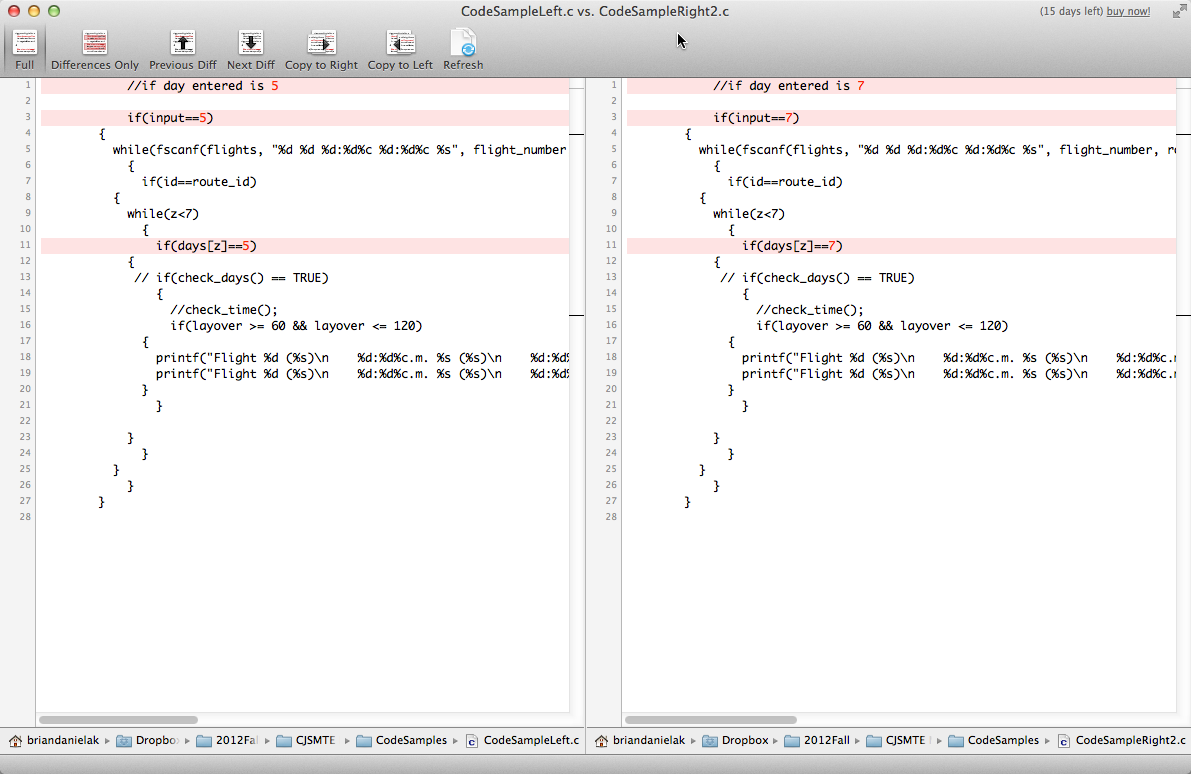
\includegraphics{media/media/image3.png}the right, and in the figure lines have been renumbered (from 1) to ease comparison. In this delta view, lines that differ are highlighted in pale red, and characters that differ are shown in bold red.

The two code blocks demonstrate just how much code is duplicated for handling user input based on days of the week. Between these two chunks there are only three differences (lines 1, 3, and 11): all of the references to day are changed from 5 (on the left) to 7 (on the right).\footnote{In the text-input files students were given, days of the week were represented as integers (rather than the perhaps more familiar ``Tuesday,'' ``Wednesday,'' etc.).} Moreover, the changes from block to block are patternistic and predictable: the first line of the block is a non-functioning comment, the third line of each block just checks whether the rest of the block should run, while the eleventh line of each block compares an array entry to the day of interest. Everything else is duplicate boilerplate that is essentially repeated 7 times; once for each day of the week. I say ``essentially repeated'' because, as we'll now explore, there are minute differences between some of the code chunk's seven incarnations.

Repeating code as Rebecca has done can be problematic because each repetition multiplies the number of places she has to examine and modify if she wants to introduce a systematic change. If, for example, Rebecca wanted to change the internal names she gives to scanned-in variables, she has to make that change in seven different blocks of code: once for each of the seven days of the week she's hard-coded. And, since any given change may inadvertently introduce an error, increasing the number of places she repeats code also makes the code that much more vulnerable to inconsistently-applied changes.

Indeed, a repeated, inconsistently-applied scan pattern change seems to be exactly what occurred in Rebecca's code history. Between 10:04pm and 10:37pm on March 26, Rebecca introduced a large set of changes to the one-stop flight module. Among those changes Rebecca added the \texttt{d\textbackslash{}\_letter} file-scanning-parameter to what would become line 218, but not to what would become line 190. We can reasonably infer Rebecca added this parameter as a way of capturing the ``am'' or ``pm'' specifier given the input file's format. Moreover, we can verify through Git that once introduced, Rebecca's omission of the parameter was never modified or corrected. The problem percolated through to her final submitted code.

\section{Augmenting Code Snapshots with Interview Data}\label{analysis-augmenting-code-snapshots-with-interview-data}

In the previous section, I described two unusual features of Rebecca's code for searching one-stop flights:

\begin{enumerate}
\def\labelenumi{\arabic{enumi}.}
\item
  Her use of multiply nested loops that scan through source information files \emph{without} storing the information in those files persistently in long-term memory

  The code for handling a user's chosen day, which was essentially the same block of code copied and pasted 7 times
\end{enumerate}

In this section, I offer explanations of Rebecca's design choices by interpreting data from over five hours of clinical interviews I conducted with her. I draw from those interviews to explain how design decisions that might seem unusual to an expert in fact grew rather unproblematically (for Rebecca) as ways of deliberately transferring prior knowledge and designs (which explains feature 1) or coping with a constraint to produce a reliable solution she could trust (which explains feature 2).

\subsubsection{Rebecca employed fscanf loops because she was deliberately reusing from an Basic Programming Assignment.}\label{rebecca-employed-fscanf-loops-because-she-was-deliberately-reusing-from-an-basic-programming-assignment.}

Rebecca's choices become easier to understand when we consider what she said in  interviews about the code she wrote. My first opportunity to discuss that code was on March 16, 2012, in what would be her third of five interviews that semester. This interview was conducted very early into the time window for the Flight Database project, before Rebecca had done the bulk of her coding. We were discussing her prospective design plans. As Rebecca began explaining how the logic for a one-stop flight search was supposed to work, she described what she saw as one of the central difficulties of the project: the relevant information for answering user queries was spread across multiple files (Interview, March 16, 2012).

As Rebecca explained, something as simple as finding a flight from, say, JFK to BWI ``involves scanning through multiple files, because it's not like one file that has everything conveniently like, there'' (Interview, March 16, 2012). When I asked what would make things easier if, hypothetically, all the information she needed were in one file, Rebecca responded by appealing to a previous assignment from last semester. In Rebecca's first-semester programming course (Basic Programming for Engineers), one of several multi-week projects had students create a system for users to conduct a fantasy football draft. The project involved, among other things, topics related to basic file management in the C language, including how to read in a file from disk (Interview, March 16, 2012). Rebecca explained:


\begin{quote}
  Rebecca: Um, like, cuz when we first got this project, uh, I actually was thinking ``oh, well this is just a lot like our fantasy football project we did last year.'' /Huh/ We uh, had to scan in, uh, someone had to enter like ``I wanna pick a quarterback,'' so then you had to scan in and go and look for all the quarterbacks in the file and say ``OK, this is the quarterback'' and everything. But, in that project we only had the one file that had everyone listed: quarterbacks, runningbacks, wide receiver, in one file. And all the information you needed there /Mmhmm/ So, you could just get it all and compare it all at once with one scanf /mmm/ whereas this you have to, take, uh, you scan in the flights, ah, the flights file. So, then you find the flight number. You have to save the ID from that flight number, use that ID to scan into the routes file /mmhmm/ and then save the routes information and then print it out with the flights information. (Interview, March 16, 2012)
\end{quote}


Rebecca's comments suggest she saw a coupling between the arrangement of the input information and the structure (and complexity) of the computational logic needed to process it. When one fantasy football file contained all of the relevant information (player, position, team, etc.) it could be read in and processed one line at a time. When information was fractured across files (pairs of airport codes in one file, full spell-outs of airport names in another, for example), Rebecca felt she'd need to use information shared across files (such as a route ID) to coordinate a scan across one file with a scan across another (and possibly an additional scan across a third file) before she would have all the necessary information and computations to return a result.

I was interested in the connections Rebecca saw across projects, so I pressed on. When I asked whether she thought about trying to make this project like her fantasy football project, her answer was an emphatic ``Oh yeah, definitely!'' As she elaborated:

\begin{quote}
  Rebecca: That was like, as soon as we got this project I was like, ah! fantasy football! I'm just gonna go and see how much code I can rework from that and like, use /mmhmm/ in this project. And, my whole main file, like all those NULL checks and everything, I mean they're really simple to write, but I just copied `em and put `em there, cuz, we had the same thing. /Mmhmm/ Um, just changed, like, the names of the files.
\end{quote}

As she explained, ``reading in files'' was a topic covered extensively in Basic Programming---the first course of the sequence---but they hadn't talked much about it in this semester's course.

\begin{quote}
  Rebecca: Because reading in from files was a big Basic Programming topic we hadn't talked about it much. /Yup/ So, I just, uh, went back to check how I did that /mmhmm/ and then, if I could I copied, but because a lot of the variables were different, uh, like these were more var---less, less variables, and more strings than last year /mmhmm/ uh, I just retyped it out. I just looked at how it was similar. (Interview, March 16, 2012)
\end{quote}

In sum, then, Rebecca's repeated, nested scan loops were a structure she deliberately borrowed from a previous semester's project. By her telling, what seemed obvious was that ``scanning in from files'' was a topic she'd already covered, which meant she'd already developed a workable solution for how to solve that problem. Thus, she saw the problem of how to coordinate airport information from different files as a new instance of the old problem of reading information in from one file. Her flight database work, accordingly, tried opportunistically adapting a previously working solution to fit the current circumstances.

\subsubsection{Rebecca repeated code because she wanted to re-use functionality she could trust}\label{rebecca-repeated-code-because-she-wanted-to-re-use-functionality-she-could-trust}

By our interview on April 6, Rebecca had already completed and submitted her code for the flights database project. When I looked at the final form of her code for finding one-stop flights I noted an unusual pattern described in section 2.4.3 above: she had a code chunk repeated almost character-for-character 7 times. In the interview, this section is what Rebecca referred to as ``my obnoxiously long part of my code'' (Interview, April 6, 2012):

\begin{quote}
  Rebecca: So, the way I did it was really long and probably, there was probably like a much easier way, but I just did a giant if---if statements \{swings cursor from line 50 to line 63\} If they wanted to fly on Monday /OK/ I went through and checked to see if the route ID was the same \{wiggles cursor across line 54\}, and if it did, I went through to che---uh, I made a check\_days function \{wiggles cursor across line 60\} uh, I ended up commenting that out cuz I didn't end up /mmhmm/ finishing it. But, uh, my check\_days function worked, it just didn't work completely with the code /OK/ (Interview, April 6, 2012)
\end{quote}

As I scrolled the screen to look at each of the repeated blocks of code, Rebecca elaborated:

\begin{quote}
  Rebecca: And this is why my code, I feel like, is not uh, concise enough, or, I don't really, I forget the word they use, but uh /\{inaudible\}/ it's very long because I couldn't figure out if I should do a while loop or whatever /Uh-huh/ But, so I was just like, I know this way should work if I get everything else right, that uh, just go through, if input's 1, if input's 2 and just do the same thing in each of `em just /Mmmhmm/ check for, ``oh, if days is 2, if days is 1'' instead of, like---Cuz I probably could have done, like, maybe a giant while loop, um, to try and, and if, while, inputs something, uh, then you check to see whatever i is. But, I could, I didn't---couldn't figure out how that would work, so I just did the same thing six times.

  Interviewer: So, in, in each one of these it's like, looks, and I'm not sure about this, but it looks like the way you wrote it---so this \{highlights line 79\} is pretty much the same in all of them, right? /Yes/

  Interviewer: So's this one \{highlights line 81\} /Yes/ this one \{highlights line 83\} Here's where it's different \{highlights line 85\}

  Rebecca: Yes, because it just checks if it's a 2 instead of a 1.

  Interviewer: OK. Um. /And then everything else is still the same/ Layover's still the same. OK.

  Rebecca: Yeah. So that's why it's prob---it's not, uh, the neatest code or whatever, because it's the same thing six times. (Interview, April 6, 2012)
\end{quote}



Given Rebecca's assertions that her code wasn't neat, I asked what, if anything she might change if she hypothetically had another week to work on the project.

\begin{quote}
  Rebecca: Um, first I'd try and get it to make sure it worked completely /Ahh, OK, yeah/ this way, \{laughs\}, uh, and then, if I had the week after that whatever, I'd probably go through and see if I could figure out a way to make it concise-r because he likes uh, neat, as, like, code that's, uh, easy for the user to see /uh-huh/ I guess. Uh, I forget what, I keep forgetting what the word he used was at the beginning of the year, but uh, just very concise and, uh, this is a very expanded \{laughs\} way of coding, but, it made sense to me at the time and I was just like ``I just want something that makes sense right now.'' /Right/ So, that I can actually work with and have an idea.

  Interviewer: Um, OK. So, so it would take you some extra thinking to figure out /Mmmhmm/ how to break this down into /Yes/ smaller stuff /smaller code/ Do you feel like you've had a lot of practice doing that, or like?

  Rebecca: Uh, a little. Like, but, a lot of times in Basic Programming they didn't really mention too much about being concise. They were just like ``if you can do it, do it'' \{laughs\} /OK/ So I usually stuck to what made sense to me /Right/ uh, to turn the projects in. (Interview, April 6, 2012)
\end{quote}

\begin{figure}[htbp]
\centering
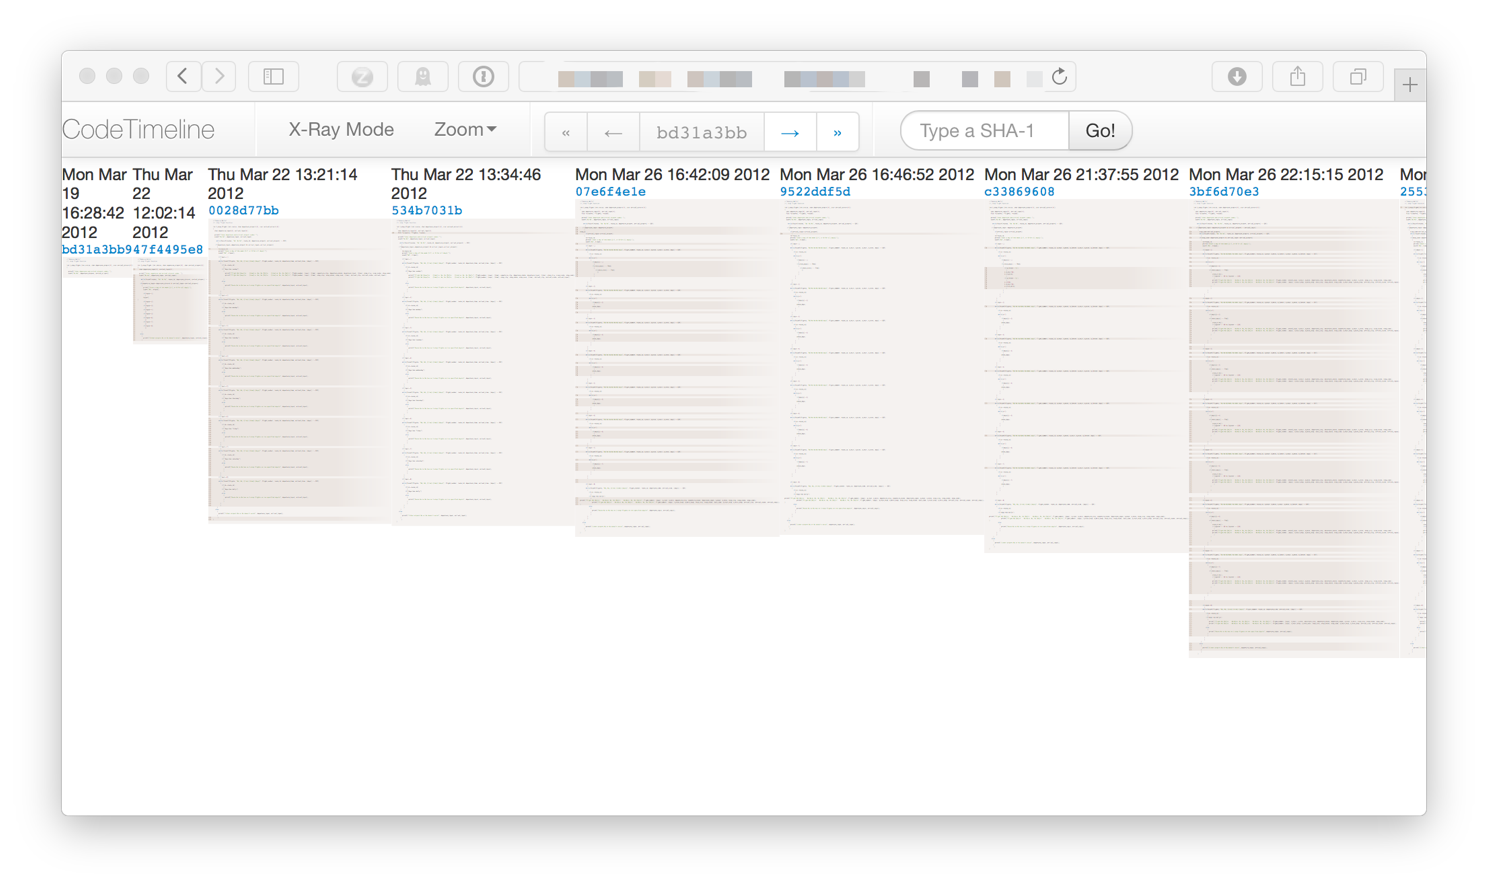
\includegraphics{media/CodeTimeline.png}
\caption{We developed CodeTimeline to display snapshots in a timeline. Darkened lines reveals how the seven-fold repeated code began as a very simple switch statement but grew and grew in complexity over time.}
\end{figure}

In summary, Rebecca's ``expanded way of coding'' was a way of expressing ideas in code that, in her own words, ``made sense'' to her. Moreover, her Basic Programming course seemed, to her, to set expectations that functionality comes first; ``neatness'' second. If she hypothetically had more time to work on the project, her first priority would be to get her existing code working. Consequently, Rebecca's repetition of code can be understood as a kind of pragmatic solution to a difficult problem: choosing which computational techniques were best for accomplishing a complex goal. Moreover, her approach was shaped by the fact that her Basic Programming course historically valued a philosophy of ``if you can do it, do it'' (Interview, April 6, 2012). Ultimately, those factors seem to be what led Rebecca to choose repeating code that made sense to her over the difficult-to-envision alternative of a ``giant while loop.''

\section{Conclusion}

Our interview with Rebecca corroborates the snapshot evidence that
Rebecca directly copied code from a prior project. Moreover, Rebecca's
behavior of copying her old fantasy football code suggests several
implications.

First, Rebecca's ``design
inertia'' actually traces as far back as the decisions she made during
the first project of her first semester of programming. That is, by
copying code (and particularly file-scanning logic) from an old project,
she was incorporating core functionality that she designed when she
first learned to program. Admittedly, code reuse isn't in and of itself
a problem in software development. \cite{parsons_cognitive_2004} Parson and Saunders for
example, have written on cognitive heuristics that keep professional
software engineers from reusing code, even when reusing and extending
existing software artifacts is the best course of action on a software
project. So, the concern isn't that Rebecca reused code, but rather the
matter of what cognitive dynamics were at play that directed her choice
to reuse that code. In that regard, the constructs of framing and
transfer may help us better understand Rebecca's activity.

Framing, as it has been applied in contexts such as physics education
\cite{elby_epistemological_2010,hammer_resources_2005,scherr_student_2009} and
mathematics education \cite{vandesande_achieving_2012}, concerns how
participants understand the social and intellectual activities in which
they're engaged. Of particular relevance to studying Rebecca is the
notion of \emph{epistemological framing}, which van de Sande and Greeno
summarize as

\begin{quote}
  participants' understanding of kinds of knowledge that are relevant for
  use in their activity and the kinds of knowledge, understanding, and
  information they need to construct to succeed in their activity (e.g.,
  what kind of information would count as a solution to the problem they
  are working on). \cite{vandesande_achieving_2012}
\end{quote}

Rebecca's decision to copy code from fantasy football implicitly
reflects her orientation toward what kinds of knowledge (the course
topic of scanning information from files) are relevant to solving the
problem. More broadly, note that in Rebecca's interview she explains
that her primary objective is to get a solution that works, which stands
in contrast to having a design priority like having a solution that is
elegant, or one that transparently manages complexity. That commitment
again reflects a manifestation of epistemological framing as ``what
would count as a solution,'' where for Rebecca what counts is a solution
that works.

Additionally, Rebecca saw the flight database project as a new instance
of a prior problem: fantasy football. Consequently, she consciously
adapted past solution patterns, because the flights database project
looked like it contained problems she had already solved in previous
code. Rebecca's deliberate reuse of old code can be readily understood
as an example of what Schwartz, Chase, and Bransford \cite{schwartz_resisting_2012} call
``overzealous transfer'':

\begin{quote}
  Of particular concern are situations where students transfer skills,
  knowledge, and routines that are effective for the task at hand but may
  nevertheless be sub-optimal in the long run because they block
  additional learning. We will call this \emph{overzealous transfer}
  (OZT)---people transfer solutions that appear to be positive because
  they are working well enough, but they are nevertheless negative with
  respect to learning what is new. \cite{schwartz_resisting_2012}
\end{quote}

In short, when students overzealously transfer prior knowledge as
Rebecca did, ``they may believe they are doing the right thing, and
without appropriate feedback they cannot know otherwise'' \cite{schwartz_resisting_2012}

In Rebecca's case, the constructs of framing and overzealous transfer
together let us describe why she would have repurposed a solution that
she felt was adequate, even to the exclusion of the topics being taught
in class and the explicit directions in the project brief. By framing
the flights database problem as a new instance of an old problem,
Rebecca treated it as she did the old problem. But, she arguably
transferred \emph{too} \emph{much} of the old code's structure; so much
that she had to introduce even more complexity into her code just to
make the transferred parts work properly under the new constraints. And,
because her framing of the task seemed to privilege a philosophy of ``if
you can do it, do it'' (Interview, April 6, 2012), her primary goals
were to get her program to work, by whatever means she could understand
and trust.

\section{Acknowledgments}\label{acknowledgments}

Blinded for review.

\clearpage

\bibliographystyle{acm}
\bibliography{bibliography}


\subsection{Acknowledgments}\label{acknowledgments}

Blinded for review.

\clearpage

\bibliographystyle{acm}
\bibliography{bibliography}

\end{document}
